\documentclass[12pt]{article}
\usepackage[margin=1.0 in]{geometry}
\addtolength{\topmargin}{.25in}
\usepackage[utf8x]{inputenc}  
\usepackage{amsmath}
\usepackage{calc}
\usepackage{array}
\usepackage{amssymb}
\usepackage{tikz}
\usetikzlibrary{arrows}
\usetikzlibrary{positioning}
%\usepackage{pgfgantt}
\usepackage{hyperref}
\usepackage{graphicx}
\usepackage{upquote}
\newcommand{\HRule}{\rule{\linewidth}{0.5mm}}
\usepackage{hyperref}
\newcommand{\Green}{\tikz\draw[green,fill=green] (0,0) circle (1 ex);}
\newcommand{\Lime }{\tikz\draw[brown,fill=brown] (0,0) circle (1 ex);}
\newcommand{\Blue}{\tikz\draw[blue,fill=blue] (0,0) circle (1 ex);}
\newcommand{\Yellow}{\tikz\draw[yellow,fill=yellow] (0,0) circle (1 ex);}
\newcommand{\Red}{\tikz\draw[red,fill=red] (0,0) circle (1 ex);}
\renewcommand*\contentsname{Indholdsfortegnelse}
\definecolor{listinggray}{gray}{0.9}
\usepackage{listings}
\lstset{
	language=C,
	literate=
		{æ}{{\ae}}1
		{ø}{{\o}}1
		{å}{{\aa}}1
		{Æ}{{\AE}}1
		{Ø}{{\O}}1
		{Å}{{\AA}}1,
	backgroundcolor=\color{listinggray},
	tabsize=3,
	rulecolor=,
	basicstyle=\scriptsize,
	upquote=true,
	aboveskip={1.5\baselineskip},
	columns=fixed,
	showstringspaces=false,
	extendedchars=true,
	breaklines=true,
	prebreak =\raisebox{0ex}[0ex][0ex]{\ensuremath{\hookleftarrow}},
	frame=single,
	showtabs=false,
	showspaces=false,
	showstringspaces=false,
	identifierstyle=\ttfamily,
	keywordstyle=\color[rgb]{0,0,1},
	commentstyle=\color[rgb]{0.133,0.545,0.133},
	stringstyle=\color[rgb]{0.627,0.126,0.941},
}
\begin{document}
\begin{titlepage}
\begin{center}

\textsc{\Large Bachelor Thesis \\ Optimized pattern matching in genomic data\\[0.3cm]}
\HRule \\[0.4cm]
{ \LARGE \bfseries Report}\\[0.4cm]
\HRule \\[1.2cm]
\textsc{\large Martin Westh Petersen - mqt967 \\ Kasper Myrtue - vkl275}\\[1.0cm]
\end{center}
\begin{center}
\vfill
{\large 20. April 2015}
\end{center}
\end{titlepage}
\tableofcontents \newpage

\section{Analysis}
\section{Loose\_match}
All possibilities are tried out using mismatches, insertions, deletions in that order to accept chars that don't match.
When all mismatches, insertions and deletions are used, and we still encounter a mismatch, the stack is popped, to
try a different order of the mismatches, insertions and deletions tried.
\subsection{Scan For Matches}
In order to understand what is good from Scan for matches we needed to understand some code segments and the overall structure of the program, simply put we came to understand this flow in the code: \\
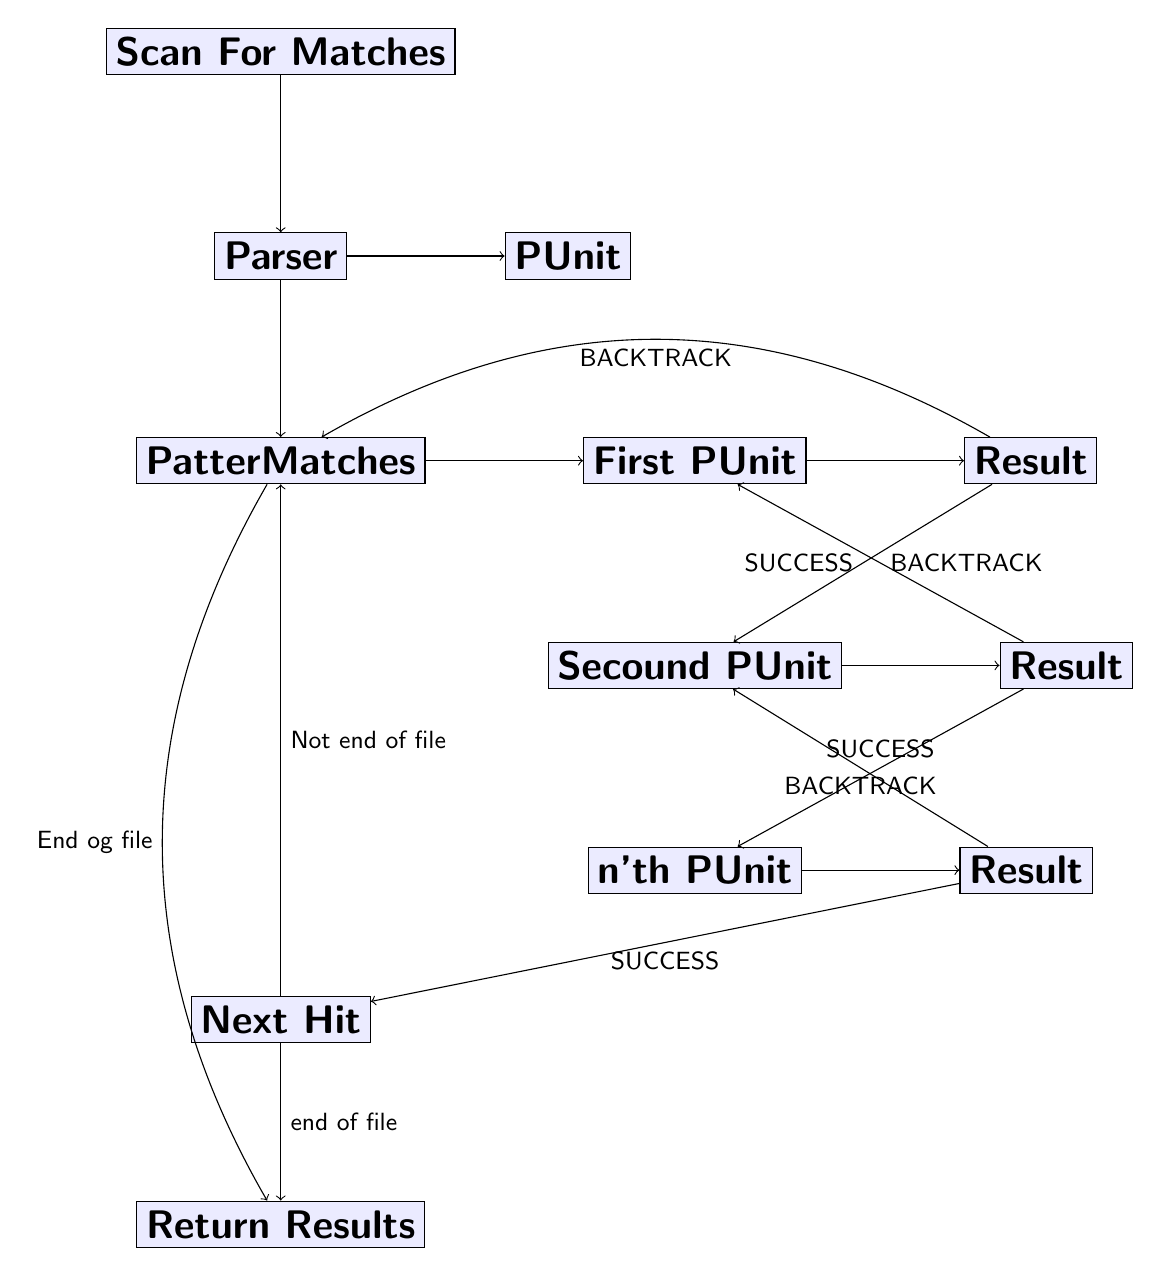
\begin{tikzpicture}
  [->,node distance=2cm and 2cm,main node/.style={rectangle,fill=blue!8,draw,font=\sffamily\Large\bfseries}] 
  \node[main node]  	(ScanForMatches)                        {Scan For Matches};
  \node[main node] 	(Parser) [below= of ScanForMatches]   {Parser};
  \node[main node] 	(PUnit) [right= of Parser]   {PUnit};
  \node[main node]  	(PatternMatch)  [below= of Parser]  {PatterMatches};
  \node[main node]	(PUnit1)		[right= of PatternMatch] {First PUnit};
  \node[main node]	(PUnit2)		[below= of PUnit1] {Secound PUnit};
  \node[main node]	(PUnitn)		[below= of PUnit2] {n'th PUnit};
  \node[main node]	(Result1)		[right= of PUnit1] {Result};
  \node[main node]	(Result2)		[right= of PUnit2] {Result};
  \node[main node]	(Resultn)		[right= of PUnitn] {Result};
  \node[]			(toNextHit)		[below= of PatternMatch] {};
  \node[	]			(to2NextHit)		[below= of toNextHit] {};
  \node[main node]	(NextHit)		[below= of to2NextHit] {Next Hit};
  \node[main node]	(Return)			[below= of NextHit] {Return Results};
  
  
  \path[every node/.style={font=\sffamily\small}]
    (ScanForMatches) 	edge node [left] {} (Parser)
    (Parser) 			edge node [left] {} (PUnit)
        					edge node [left] {} (PatternMatch)
    (PatternMatch) 		edge node [left] {} (PUnit1)
    						edge [bend right] node [left] {End og file} (Return)
    (PUnit1) 			edge node [left] {} (Result1)
    (PUnit2)				edge node [left] {} (Result2)
    (PUnitn)				edge node [left] {} (Resultn)
    (Result1)			edge node [left] {SUCCESS} (PUnit2)
    						edge [bend right] node [below] {BACKTRACK} (PatternMatch)
    (Result2)			edge node [above] {SUCCESS} (PUnitn)
    						edge node [right] {BACKTRACK} (PUnit1)
    (Resultn)			edge node [below] {SUCCESS} (NextHit)
        					edge node [below] {BACKTRACK} (PUnit2)
    (NextHit)			edge node [right] {Not end of file} (PatternMatch)
        					edge node [right] {end of file} (Return)
    ;
    
\end{tikzpicture} \\
This shows how Scan\_For\_Match uses a backtrack algorithm to search trough the data. When ever a PUnit fails it calls BACKTRACK, a case in the function patternMatch in Scan\_For\_Match. \\

We have found certain structures he uses to solve different functionality problems, in order to harvest these structures to achieve the same fast runtime in the base cases of the program (e.g. exact match for bases or the like) we need to understand them:

\subsection{Ambiguous bases}
In Scan\_For\_Match in order to compare strings of bases he needs to be able to compare with bases that can mean different other bases, (e.g. n is way to write (A or C or T or G), and m is a way of writing (A or C)) this is done by converting all bases to words of 4 bit. This makes it possible to use bit wise and to compare bases. \\
in order to do this we need to define the different bases as 1 bit being true (e.g. A = 0001, C = 0010 ....) this makes it possible for ambiguous bases to say which bases it consists of. In Scan\_For\_Match he has made a conversion table for this:
\begin{lstlisting}
int build_conversion_tables()
{
    int the_char;

    for (the_char=0; the_char < 256; the_char++) {
        switch(tolower(the_char)) {
          case 'a': punit_to_code[the_char] = A_BIT; break;
          case 'c': punit_to_code[the_char] = C_BIT; break;
          case 'g': punit_to_code[the_char] = G_BIT; break;
          case 't': punit_to_code[the_char] = T_BIT; break;
          case 'u': punit_to_code[the_char] = T_BIT; break;
          case 'm': punit_to_code[the_char] = (A_BIT | C_BIT); break;
          case 'r': punit_to_code[the_char] = (A_BIT | G_BIT); break;
          case 'w': punit_to_code[the_char] = (A_BIT | T_BIT); break;
          case 's': punit_to_code[the_char] = (C_BIT | G_BIT); break;
          case 'y': punit_to_code[the_char] = (C_BIT | T_BIT); break;
          case 'k': punit_to_code[the_char] = (G_BIT | T_BIT); break;
          case 'b': punit_to_code[the_char] = (C_BIT | G_BIT | T_BIT); break;
          case 'd': punit_to_code[the_char] = (A_BIT | G_BIT | T_BIT); break;
          case 'h': punit_to_code[the_char] = (A_BIT | C_BIT | T_BIT); break;
          case 'v': punit_to_code[the_char] = (A_BIT | C_BIT | G_BIT); break;
          case 'n': punit_to_code[the_char] = (A_BIT | C_BIT | G_BIT | T_BIT); break;
          default:
            punit_to_code[the_char] = 0;
            break;
        }
        if (punit_to_code[the_char] & A_BIT)
            punit_to_code[the_char] |= T_BIT << 4;
        if (punit_to_code[the_char] & C_BIT)
            punit_to_code[the_char] |= G_BIT << 4;
        if (punit_to_code[the_char] & G_BIT)
            punit_to_code[the_char] |= C_BIT << 4;
        if (punit_to_code[the_char] & T_BIT)
            punit_to_code[the_char] |= A_BIT << 4;
    }
...
\end{lstlisting}

This makes him able to use bit wise and to determine a match in the following way:
\begin{lstlisting}
#define KnownChar(C)  (punit_sequence_type == PEPTIDE ? 1 : known_char[(C)])

#define Matches(C1,C2) (punit_sequence_type == PEPTIDE ? \
                        ((C1 == C2) || (C2 == 'X')): \
                        (KnownChar((C1) & 15) && ((((C1) & 15) & ((C2) & 15)) == (C1 & 15))))

\end{lstlisting}
In the code segment above C1 is a character from the data and C2 is a character from the pattern given. In the case where it is not PEPTIDE (PEPTIDE being not DNA) he starts by checking that the data character is a allowed base, if this is true and the two characters being bit wise "and" compared results in the same word taken from the data, it returns true. 

When he grabs the two characters to compare, he doesn't just get 4bits in order to make sure it is only the 4bits he is interested in, that gets compared he bit wise "and" them with 15. This makes all other than the last 4 bits go to 0 because 15 is 4 ones in end of the Bite.

The smart result of this comparing algorithm is that you only need to compare once even though the pattern can have multiple different ambiguous bases. It will always return the base from the data if the ambiguous base contains the base from the data. example: \\
\begin{itemize}
\item The base from the data is: A (0001)
\item The ambiguous base from the pattern is: D (A or T or G) 1101
\item The bit wise "and" operation: 0001 \& 1101 = 0001
\item The result is then compared with A again to see if the compare was successful
\end{itemize}
In order to use this he has converted both the data and the pattern with the conversion\_table. \\
\section{Design}

\subsection{Program structure}

A list of actions our program should do in order to execute a pattern search:
\begin{itemize}
\item Read and parse the input line. E.g. "scanFM 'ATTGCCCC[0,1,2]' 'data.txt'". Possibility of writing "$->$ 'output.txt'"
which results in the matches not being displayed in the terminal but written the the specified file.
\item Parse the pattern into units and save them as different types (objects of different classes that inherit
from a common PUNIT class), e.g. EXACT\_PUNIT, AMBI\_PUNIT etc.
\item Choose the order of which to search for the patterns and create a state that readies for this search, for example a 
list of the punits in correct order with some way of keeping track of the different positions the punits have to with
respect to each other.
\item Search for the punits in the order chosen by simply calling a ".search()" method for each PUNIT-object.
The PUNIT-object's search method invoked is unique for each different type of PUNIT, and returns either True or False.
If the search for each PUNIT returns True the match is saved.
\item The saved matches are either displayed in the terminal or written in a file, depending on the call of scanFM. 
\end{itemize}


\textbf{Types of PUNITs that we need}
\begin{itemize}
\item EXACT - A PUNIT of this type consists of either of the letters 'A', 'C', 'G' and 'T' or any number of the wildcards. Also includes begin able to search with a given number of mismatches, insertions, and deletions.
\begin{itemize}
  \item The two scenarios of a exact search is either, only literals without mismatches, insertions or deletions, or literals with insertions, deletions or mismatches.
  \item Without mis, ins, and del, the algorithm runs through all the pattern bases, and compares them to all data bases with the same incrementation from a given point in the data. This means that worst case it has to run the pattern length for each data point, which gives O(n*m) worst case runtime, n being the data length, and m being the pattern length.
  \item With mis, ins and del, the search function has to do the same as before but trying with all failed matches between data and pattern to insert a mismatch, deletion or insertion. This makes the worst case runtime increase to O(n*m*ins*del*mis) since insertions, deletions and mismatches has to be tryed in all different orders.
  \item both scenarios is using the same algorithms as scan for matches.
\end{itemize}
\item COMPLEMENTARY - A PUNIT that takes the complementary of a literal.
\begin{itemize}
  \item complementary punit uses the code from exact to search, it only changes the code from the pattern to the complementary, which happens in O(m), m being the pattern length.
\end{itemize}
\item REPEAT - Saves another PUNITs result to search for it later.
\begin{itemize}
  \item repeat uses either complementary or exacts search function depending on which Punit it points to, not increasing the overall time consumption.
\end{itemize}
\item RANGE - Jumps all distances between to given parameters.
\begin{itemize}
  \item Range only jumps in the data file, which is done in constant time.
\end{itemize}
\end{itemize}

\begin{figure}[h!]
\includegraphics[scale=0.6]{UML.png}
\caption{ULM class diagram of scanfm Punits}
\end{figure}

\subsection{Optimization}
\subsubsection{Skip length}
The pattern is matched against the database sequence as usual with different orders of mismatches, insertions and
deletions if necessary, however it stores the amount of occurrences of each letter in a list, in the interval
(SR, SR + length(pattern) + insertions) (datlist). 
It also stores the amount of occurrences of letters in the pattern (patlist). \\ \\
Say there is not match in this first run. Normally we would increment the SR counter and try again, but instead we
increment SR, and update the datlist with the new letters (the old first letter is decremented and the new letter in the
end of the string in incremented in datlist). For any letter, if the number of occurrences in patlist p subtracted the
number of allowed mismatches and deletions still is bigger than the number of occurrences of that letter in dalist, there is no 
possible match between these 2 strings, in that particular search can be skipped. (Only subtract deletions if the last letter
in the DB-subsequence is not the letter being checked.) Pseudo algorithm would be as follows: 
\begin{enumerate}
\item In the first search, count the number of occurrences of each letter in pattern (put them in patlist) 
and DB-subsequence being checked, i.e. interval(SR, SR + length(pattern) + max\_insertions (put them in datlist)
; Pattern match the two strings; if succes goto 6;
\item SR++
\item Update letter occurrences in datlist
\item for each letter lt: if ((patlist[lt] - max\_mismatch) - (max\_deletions - 
NumberOfLet(lt, interval(ER - max\_deletions, ER))) $>$ datlist[lt] then goto 2;
\item Pattern match the 2 strings; goto 2;
\item DONE
\end{enumerate}
Here's an example. Suppose the DB-sequence is "$<$something before$>$ACCCTTT$<$something after$>$" and the pattern we're
looking for is "ATTTTTT[2,0,3]" (2 mismatches, 3 deletions.) For the letter "T" the check in 4 would be: \\
((6 - 2) - (3 - NumberOfLet("T", "TTT")) = ((6 - 2) - (3 - 3)) = 4. 4 is bigger than datlist("T") = 3 so there is no
possible match.

\end{document}
